\documentclass[12pt]{article}

\usepackage[utf8]{inputenc}
\usepackage[T1]{fontenc}
\usepackage[francais]{babel}
\usepackage{multirow}
\usepackage{array}
\usepackage{stmaryrd}
\usepackage{listings}
\usepackage{color}
\usepackage{amsmath}
\usepackage{graphicx}
\usepackage{titlesec}
\usepackage{titletoc}
\usepackage{fullpage}
\usepackage{multirow}

\titleformat{\chapter}[hang]{\bf\huge}{}{2pc}{}


\begin{document}

\begin{titlepage}
\begin{center}

\textsc{\LARGE IUT Belfort Montbéliard}\\[4cm]

% Title
{ \huge \bfseries Projet de Base de Données :\\[0.3em] Gestion d'une boulangerie\\[1em]Cahier des charges}\\[4cm]

% Author and supervisor
{
\begin{large}
\setlength{\baselineskip}{1.6\baselineskip}
\emph{Étudiants en charge du projet: \\[0.5em]}
\textsc{Houdayer} Benoit\\
\textsc{Ruhier} Anthony\\[2em]

\end{large}
}

\vfill

\end{center}
\end{titlepage}


	\section{Objectifs}

Apporter à l'utilisateur un assistant vocal intégré dans ses applications
préférées. Le projet sera livré le 5 février.

	\section{Description du produit}

L'application doit être capable de :
\begin{itemize}
    \item synthétiser la voix de l'utilisateur sous forme de texte;
    \item faire le lien entre les données textuelles et les fonctions
        implémentées;
    \item s'intégrer avec les applications de l'utilisateur;
    \item faciliter l'intégration avec de nouvelles applications;
    \item communiquer avec l'utilisateur via la synthèse vocale;
\end{itemize}


    \section{Grandes étapes et calendrier}

\begin{center}
{
\let\oldtabular=\tabular
\def\tabular{\normalsize\oldtabular}
\renewcommand{\arraystretch}{1.5}
\begin{tabular}{|l|c|}
	\hline
    18/10/2013 & MCD terminé.\\
	\hline
    28/10/2013 & Début du développement.\\
    \hline
    Novembre 2013 & Interface réalisée, base de donnée crée.\\
    \hline
    \multirow{2}{*}{Décembre 2013} & Site fonctionnel, design proche du rendu final, début de la phase de \\
    & corrections de bugs.\\
    \hline
	07/01/2014 & Finalisation du développement.\\
	\hline
\end{tabular}
}
\end{center}


	\section{Budget}

Aucun budget n'est à prévoir : le présent projet ne fait pas l'objet de compensation financière et les outils permettant sa conception sont déjà disponibles à titre gratuit.

    \section{Modèle conceptuel de données}


\begin{figure}[h!]
    \centering
    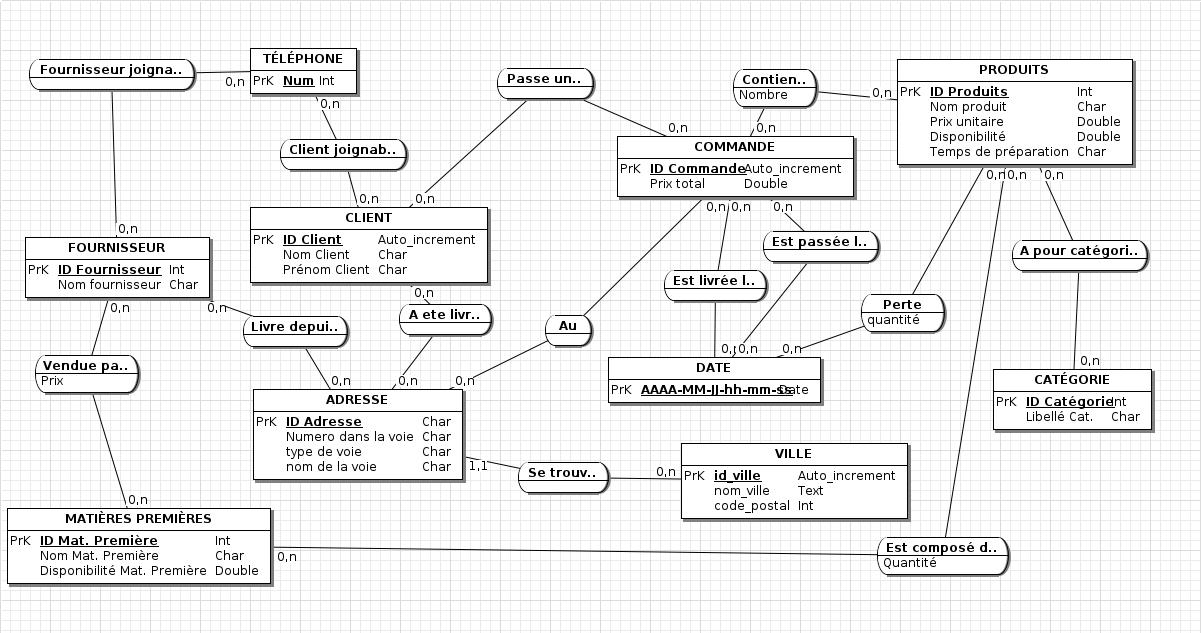
\includegraphics[width=16.5cm]{images/MCD.jpg}
    \caption{Modèle conceptuel de données}
\end{figure}
\newpage

    \section{Arbre des fonctionnalités}


\begin{figure}[h!]
    \centering
    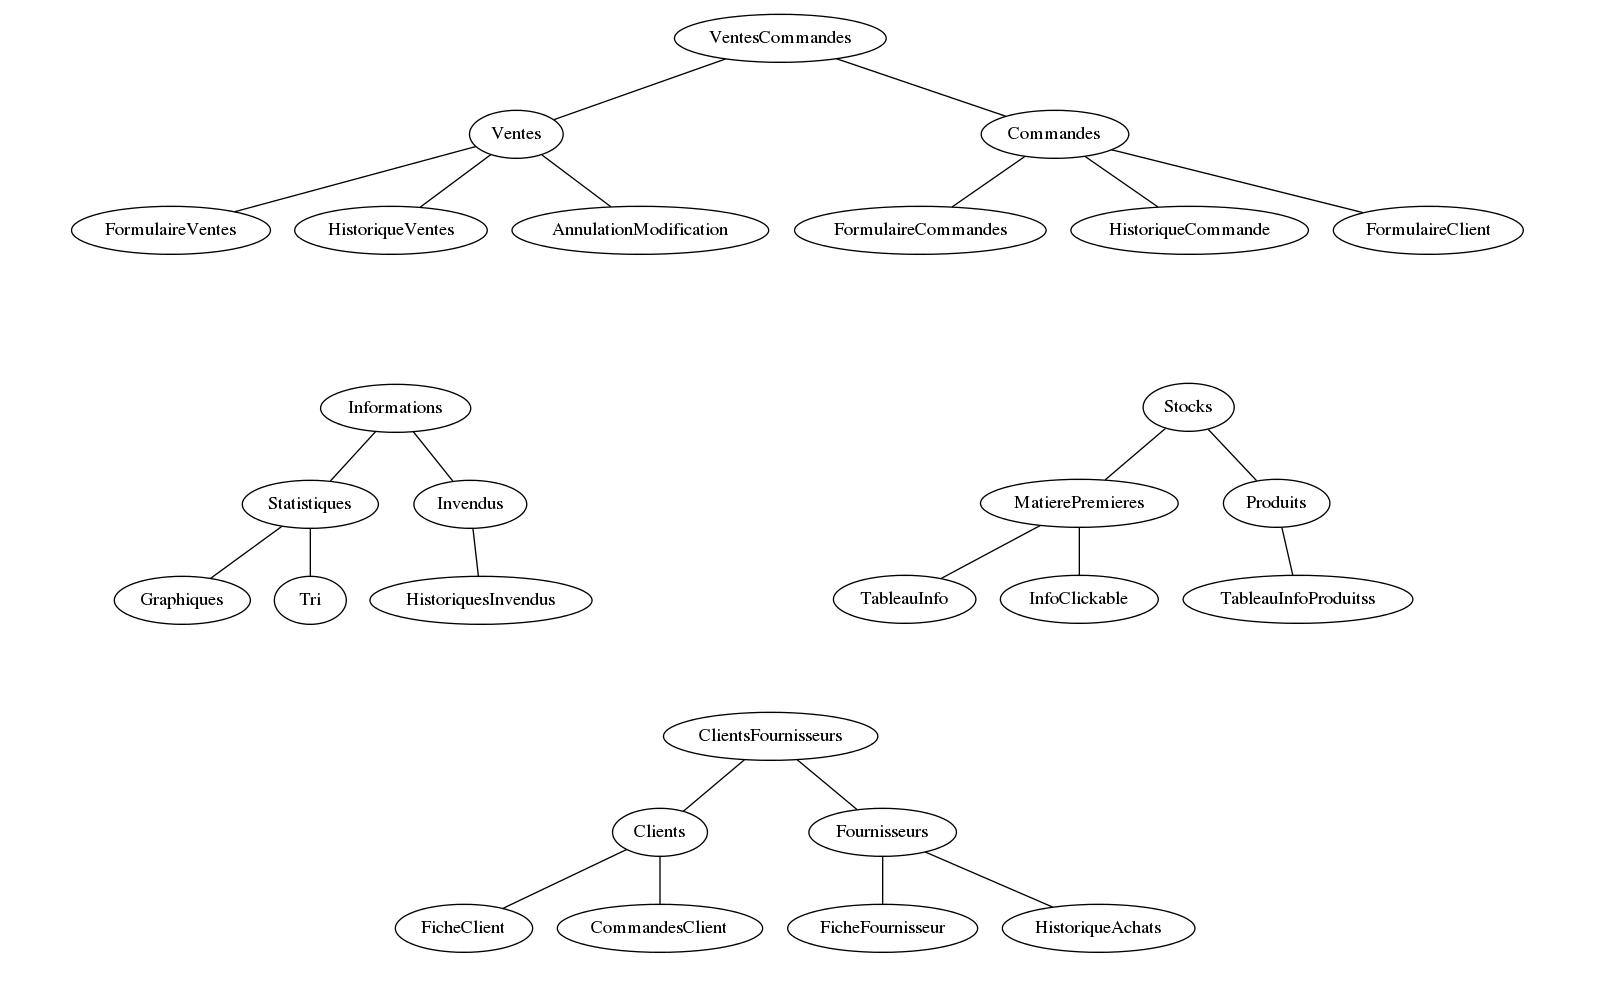
\includegraphics[width=16.5cm]{images/DHM.png}
    \caption{Arbre des fonctionnalités}
\end{figure}
\newpage

    \section{Tracé régulateur}


\begin{figure}[h!]
    \centering
    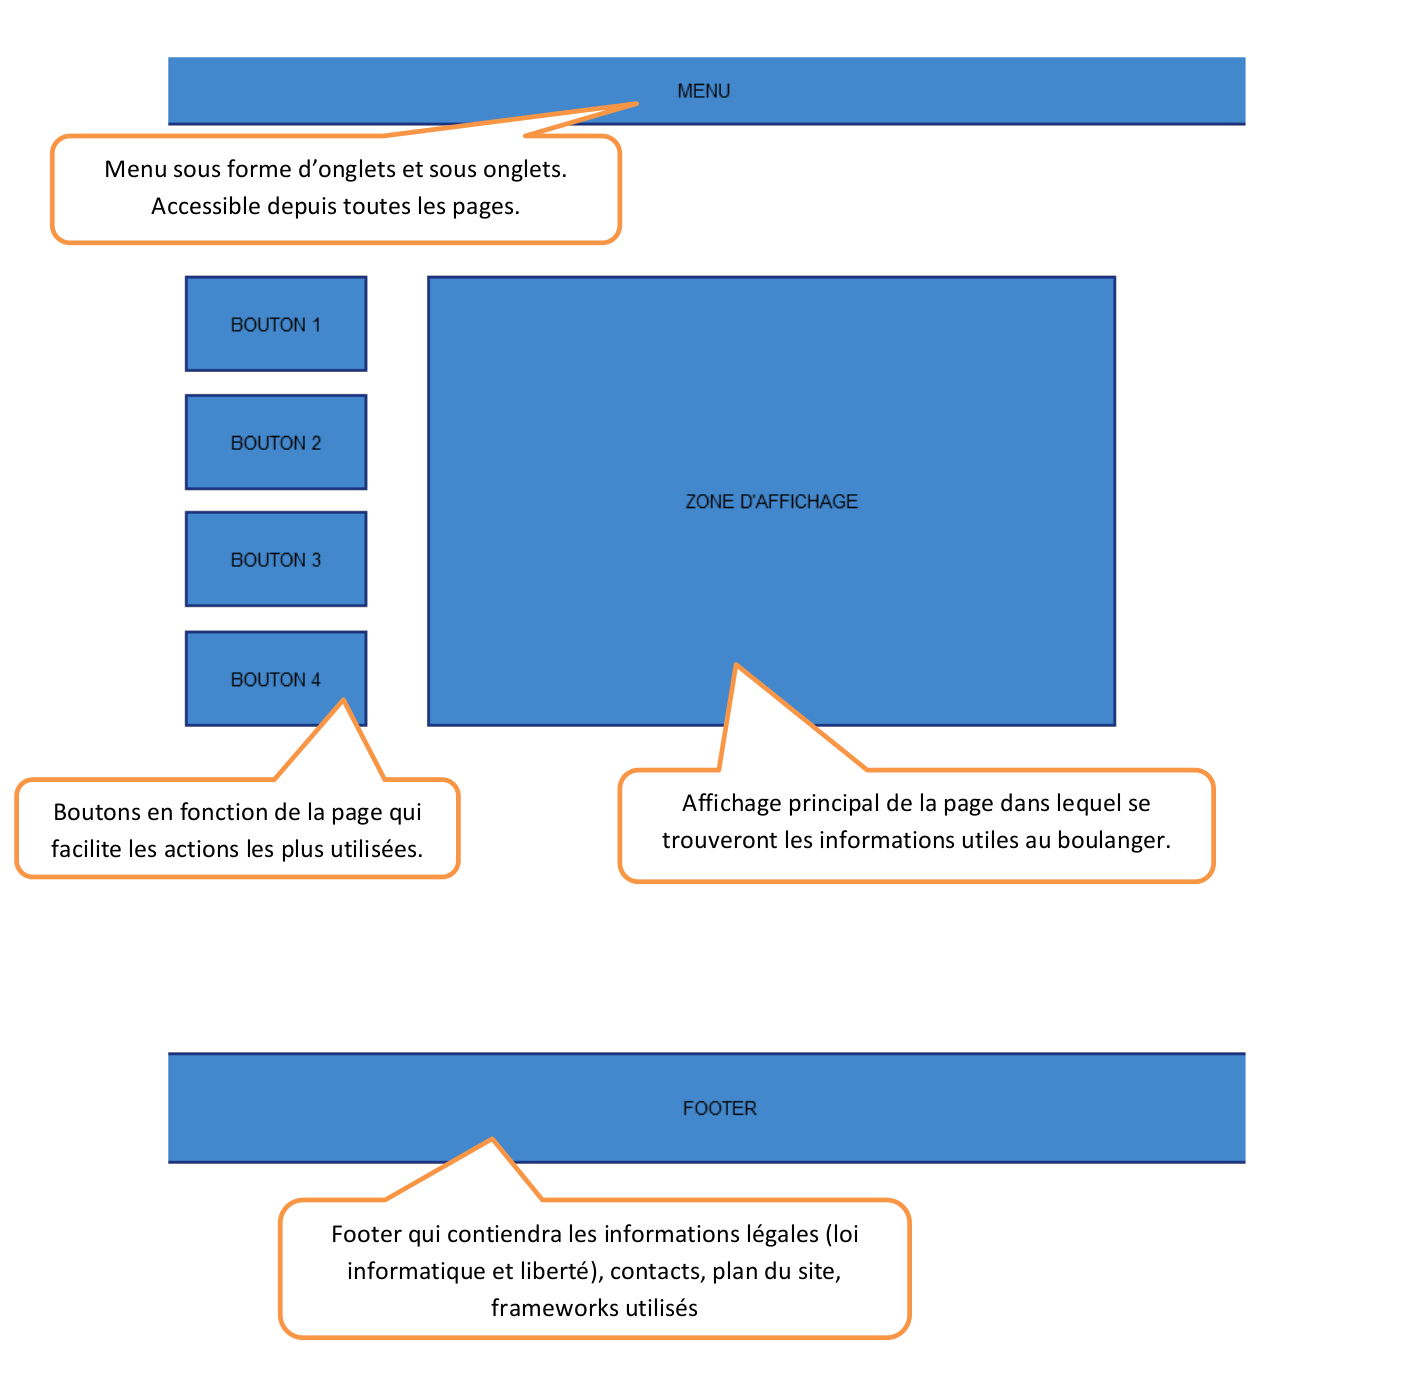
\includegraphics[width=16.5cm]{images/Trace-regulateur.png}
    \caption{Tracé régulateur}
\end{figure}

\end{document}
